\section{Discussion and conclusions}
\label{chapter:06}

% block-id: auto.06.p1
\hypertarget{auto.06.p1}{}
Reviewable automated research depends on a continuous association between tasks and evidence. Visible requests, tool events, source differences, and deterministic tests organize the execution records of the cases studied here. Scientific judgment still requires explicit model applicability, comparison quantities, and acceptance tolerances. Executable code, generated graphics, and typeset papers address software execution, result presentation, and document construction, respectively; acceptance steps connect these activities to physical reliability.

% block-id: auto.06.p2
\hypertarget{auto.06.p2}{}
The research process involves both editable and stable objects. Parameters, source, and follow-up tasks must remain easy to modify, while the inputs and results supporting conclusions are fixed by hashes. Versioned data directories preserve original file identities, and new runs use separate directories. Redrawn figures record their saved inputs and transformations. Bilingual manuscripts share equation, figure, and citation identities, allowing changes in presentation to be traced to the same scientific content.

% block-id: auto.06.p3
\hypertarget{auto.06.p3}{}
This workflow is particularly suitable for progressively richer modeling. Analytical and two-dimensional cases provide inexpensive regressions; small-strand models test common-terminal constraints; finite-length and three-dimensional routes introduce additional degrees of freedom. Saved geometry and field data retain the inputs needed for subsequent three-dimensional interpretation. Actual centerlines retain strand identity, arc length, and local position as inputs for model extension. Structural performance comparisons also require matched copper volume, return, end regions, and numerical uncertainty.

% block-id: auto.06.figure
\hypertarget{auto.06.figure}{}
\begin{figure*}[!htbp]
\centering
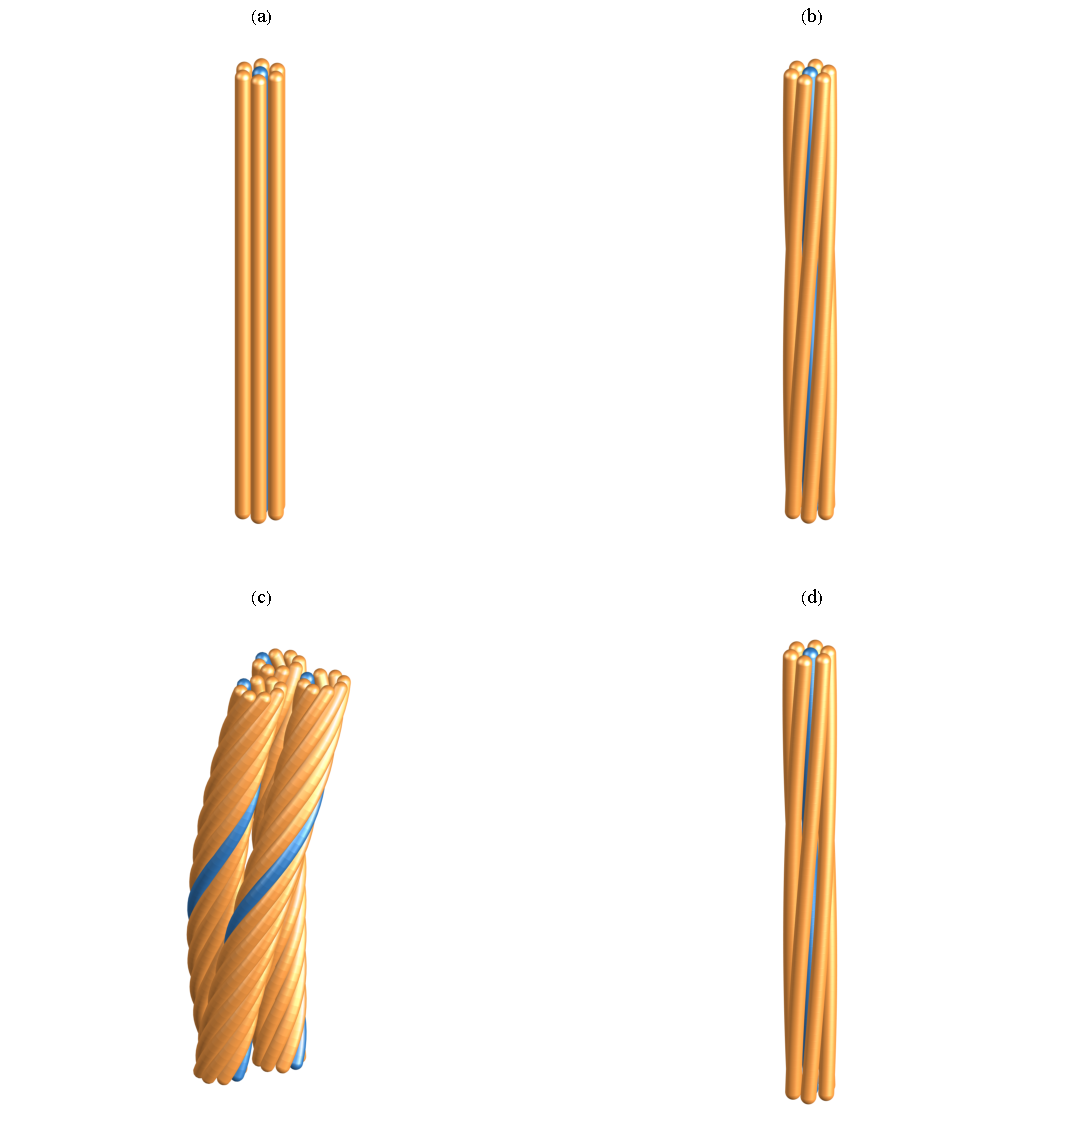
\includegraphics[width=\linewidth,height=.72\textheight,keepaspectratio]{../../assets/en/geometry_comparison.pdf}
\caption{Three-dimensional strand centerline structures. Panels show straight, single-level, local multilevel, and cross-layer structures. The 24-strand structures use a copper diameter of 0.100 mm, and the multilevel panel shows a 3 mm detail. Blue markers preserve selected physical strand identities.}
\label{fig:geometry_comparison}
\end{figure*}

% block-id: auto.06.p4
\hypertarget{auto.06.p4}{}
This work provides workflows, connection configurations, execution adapters, model source, and traceable cases. The existing records support Codex completing specified modeling tasks through Wolfram and Ansys MCP, extending an analytical implementation, and repairing an interface using error evidence. Cross-solver and A–φ cases further show how acceptance status constrains interpretation. Subsequent methodological evaluation can add independent clients, repeated tasks, and manual baselines to study completion rates, resource costs, and repair stability across task complexities.

% block-id: auto.06.p5
\hypertarget{auto.06.p5}{}
Wolfram, AgentTools, PyAEDT-MCP, PyAEDT, and associated open-source numerical and document tools support this implementation. AI assisted source inspection, model and adapter code, call orchestration, diagnostics, and manuscript preparation; the author is responsible for physical assumptions, acceptance criteria, and scientific conclusions. The repository supplies software-environment and upstream-source records, allowing readers to continue through the linked methods, implementations, tests, and results.
